\setAuthor{Hans Daniel Kaimre}
\setRound{lõppvoor}
\setYear{2018}
\setNumber{G 1}
\setDifficulty{2}
\setTopic{Geomeetriline optika}

\prob{Poolitatud lääts}
Kersti paneb kokku optilise skeemi, nii et koondav lääts on objektist ja ekraanist, kuhu terav kujutis tekib, võrdsel kaugusel. Ta jätab objekti ja ekraani asukoha samaks, kuid lõikab läätse optilise peatelje juurest pooleks ning nihutab kaks tekkinud poolikut läätse optilisest peateljest eemale. Joonistage lisalehel uue skeemi jaoks kiirte käik. Objekt on tähistatud A-ga.
\begin{center}
 \begin{tikzpicture}[scale=0.5]

 % Def. koordinaadid
 \coordinate (O) at (0,0) ;
 \coordinate (A) at (-8,0) ;
 \coordinate (A') at (8,0) ;
 \coordinate (1) at (0,2);
 \coordinate (2) at (0,6);
 \coordinate (3) at (0,-2);
 \coordinate (4) at (0,-6);
 \coordinate (K) at (-6,4);
 \coordinate (KO) at (-6,0);
 

 % Jooned, t2pid
 \draw[thick] (A) -- (A');
 \draw[thick][->] (1) -- (2);
 \draw[thick][->] (3) -- (4);
 \pgfsetarrowsstart{latex}
 \draw[ultra thick] (K) -- (KO) ;
	
 % Nurgad ja punktid
 \node[] at (-7.0,4) {A};
 
\end{tikzpicture}
\end{center}

\hint
Objekti kaugus läätsest on üheselt ära määratud sellega, et lääts on objektist ja kujutisest ühel kaugusel. Kiirte edasise käigu jaoks tuleb mõlemat läätse poolt eraldi vaadata.

\solu
Ülesande püstituses on öeldud, et esialgse skeemi korral on lääts objektist ja kujutisest võrdsel kaugusel. Selline olukord realiseerub, kui nii objekt kui ka kujutis asuvad läätsest kahekordses fookuskauguses, kusjuures süsteemi suurendus on 1(objekt ja kujutis on sama suured). Läätse poolekslõikamisel ja poolde nihutamisel joonisel toodud skeemi järgi saame kaks uut läätse, mille fookuskaugused on endiselt samad, kuid optilised peateljed on nihkes. Seega tekib ekraanile kaks samasuurt kujutist kui enne, mis on omavahel vertikaalselt nihutatud ning mille intensiivsus on võrreldes esialgse kujutisega tunduvalt vähenenud. Seejuures paneme konstrueerimisel tähele, et kuigi reaalselt läätsest väljapool olevast piirkonnast kiiri läbi ei lähe, saame neid siiski kujutise konstrueerimiseks kasutada.

\begin{center}

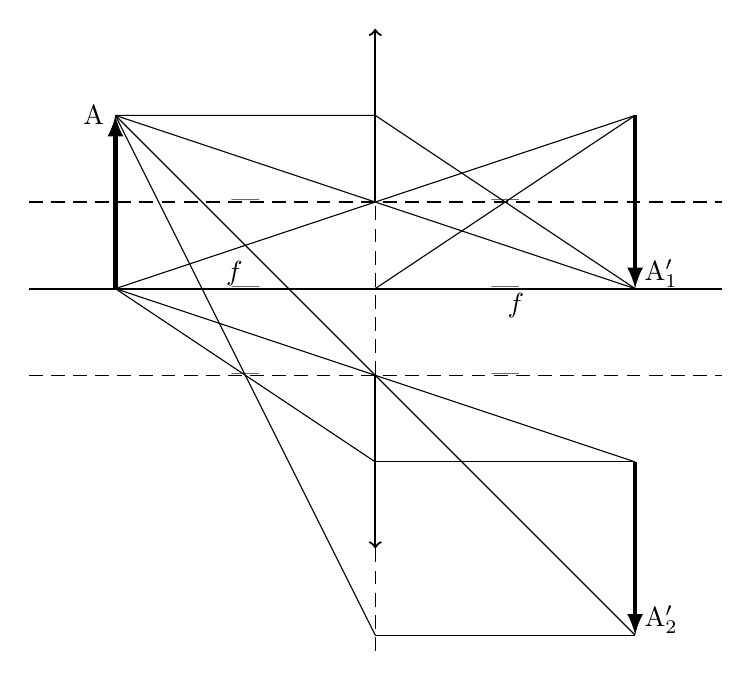
\begin{tikzpicture}[scale=0.55]

 % Def. koordinaadid
 \coordinate (O) at (0,0) ;
 \coordinate (A) at (-8,0) ;
 \coordinate (A') at (8,0) ;
 \coordinate (1) at (0,2);
 \coordinate (2) at (0,6);
 \coordinate (3) at (0,-2);
 \coordinate (4) at (0,-6);
 \coordinate (K) at (-6,4);
 \coordinate (KO) at (-6,0);
 

 % Jooned, t2pid
 \draw[thick] (A) -- (A');
 \draw[thick][->] (1) -- (2);
 \draw[thick][->] (3) -- (4);
 \draw[dash pattern=on5pt off3pt] (-8,2) -- (8,2);
 \draw[dash pattern=on5pt off3pt] (-8,-2) -- (8,-2);
 \draw[dash pattern=on5pt off3pt] (0,-2) -- (0,2);
 \draw[dash pattern=on5pt off3pt] (0, -6) -- (0,-8.5);
 \draw (K) -- (6,0);
 \draw (K) -- (0,4);
 \draw (6,0) -- (0,4);
 
 \draw (KO) -- (6,4);
 \draw (0,0) -- (6,4);
 
 \draw (KO) -- (6,-4);
 \draw (KO) -- (0,-4);
 \draw (6,-4) -- (0,-4);
 
 \draw (K) -- (6,-8);
 \draw (K) -- (0,-8);
 \draw (0,-8) -- (6,-8);
 
 \pgfsetarrowsstart{latex}
 \draw[ultra thick] (K) -- (KO) ;
 \draw[ultra thick] (6,0) -- (6,4) ;
 \draw[ultra thick] (6,-8) -- (6,-4) ;

 % Nurgad ja punktid
 \node[] at (-6.5,4) {A};
 \node[] at (-3,0) {|};
 \node[] at (3,0) {|};
 \node[] at (-3,2) {|};
 \node[] at (3,2) {|};
 \node[] at (-3,-2) {|};
 \node[] at (3,-2) {|};
 \node[] at (3.25,-0.4) {$f$};
 \node[] at (-3.25,0.35) {$f$};
 \node[] at (6.6,0.35) {$\mathrm{A_1'}$};
 \node[] at (6.6,-7.65) {$\mathrm{A_2'}$};
 
\end{tikzpicture}
\end{center}

\probeng{Split lens}
Kersti is putting together an optical diagram so that a convex lens is at an equal distance from the object and the screen, on which a sharp image forms. She lets the positions of the object and the screen be the same but cuts the lens in half at the optical axis and moves the two new split lenses away from the optical axis. Draft the directions of the rays for the new diagram. The object is marked as A.
\begin{center}
  \begin{tikzpicture}[scale=0.5]

    % Def. koordinaadid
    \coordinate (O) at (0,0) ;
    \coordinate (A) at (-8,0) ;
    \coordinate (A') at (8,0) ;
    \coordinate (1) at (0,2);
    \coordinate (2) at (0,6);
    \coordinate (3) at (0,-2);
    \coordinate (4) at (0,-6);
    \coordinate (K) at (-6,4);
    \coordinate (KO) at (-6,0);
    

    % Jooned, t2pid
    \draw[thick] (A) -- (A');
    \draw[thick][->] (1) -- (2);
    \draw[thick][->] (3) -- (4);
    \pgfsetarrowsstart{latex}
    \draw[ultra thick] (K) -- (KO) ;
	
    % Nurgad ja punktid
    \node[] at (-7.0,4)  {A};
    
\end{tikzpicture}
\end{center}

\hinteng
The object's distance from the lens is determined by the fact that the lens is at the same distance from both the object and the image. Each side of the lens should be looked at separately for the further path of the rays.

\solueng
In the problem it is said that in the original diagram the lens is at an equal distance from the object and the image. This situation is realized if both the object and the image are at double the focal length from the lens, moreover the magnification of the diagram is 1 (the object and the image are the same size). After cutting the lens in half we get two new lenses that still have the same focal lengths but the optical axes are displaced. Therefore two images appear on the screen that have the same sizes as before but the images are vertically displaced between each other and their intensities compared to the initial image are considerably smaller. While constructing we will also notice that even though realistically no rays go through the region outside the lens we can still use them in the construction of the image.
\begin{center}

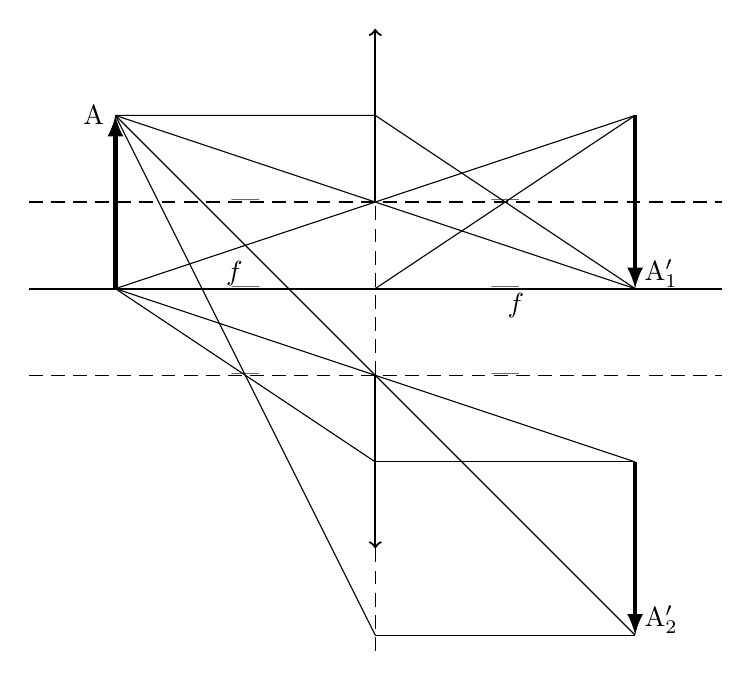
\begin{tikzpicture}[scale=0.55]

    % Def. koordinaadid
    \coordinate (O) at (0,0) ;
    \coordinate (A) at (-8,0) ;
    \coordinate (A') at (8,0) ;
    \coordinate (1) at (0,2);
    \coordinate (2) at (0,6);
    \coordinate (3) at (0,-2);
    \coordinate (4) at (0,-6);
    \coordinate (K) at (-6,4);
    \coordinate (KO) at (-6,0);
    

    % Jooned, t2pid
    \draw[thick] (A) -- (A');
    \draw[thick][->] (1) -- (2);
    \draw[thick][->] (3) -- (4);
    \draw[dash pattern=on5pt off3pt] (-8,2) -- (8,2);
    \draw[dash pattern=on5pt off3pt] (-8,-2) -- (8,-2);
    \draw[dash pattern=on5pt off3pt] (0,-2) -- (0,2);
    \draw[dash pattern=on5pt off3pt] (0, -6) -- (0,-8.5);
    \draw (K) -- (6,0);
    \draw (K) -- (0,4);
    \draw (6,0) -- (0,4);
    
    \draw (KO) -- (6,4);
    \draw (0,0) -- (6,4);
    
    \draw (KO) -- (6,-4);
    \draw (KO) -- (0,-4);
    \draw (6,-4) -- (0,-4);
    
    \draw (K) -- (6,-8);
    \draw (K) -- (0,-8);
    \draw (0,-8) -- (6,-8);
    
    \pgfsetarrowsstart{latex}
    \draw[ultra thick] (K) -- (KO) ;
    \draw[ultra thick] (6,0) -- (6,4) ;
    \draw[ultra thick] (6,-8) -- (6,-4) ;

    % Nurgad ja punktid
    \node[] at (-6.5,4)  {A};
    \node[] at (-3,0)  {|};
    \node[] at (3,0)  {|};
    \node[] at (-3,2)  {|};
    \node[] at (3,2)  {|};
    \node[] at (-3,-2)  {|};
    \node[] at (3,-2)  {|};
    \node[] at (3.25,-0.4)  {$f$};
    \node[] at (-3.25,0.35)  {$f$};
    \node[] at (6.6,0.35)  {$\mathrm{A_1'}$};
    \node[] at (6.6,-7.65)  {$\mathrm{A_2'}$};
    
\end{tikzpicture}
\end{center}
\probend